\chapter{Channel Modeling}
\section{Modeling}
As the controller is run on two different masters, a link between these have to be established and modeled. The connection is seen as a connection from a master (ex. a "mothership") and a slave (ex. AAUSHIP). Where the communication goes both ways, as the master needs to compute what the slave should do next based on measurements from the slave, and the slave needs to respond to these data. Figure \vref{fig:chanmod} is an illustration of the communication. 

\begin{figure}[htbp]
		\begin{center}
			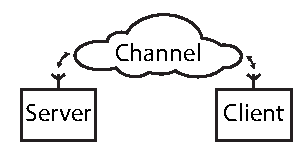
\includegraphics[width=8.4cm]{img/chanmod}
			\caption{Depiction of the communication link between the master and the slave.}
			\label{fig:chanmod}
		\end{center}
\end{figure}

As the protocol between the master and the slave, includes a validity check, the channel estimation becomes a simple question of wether or not the received package is valid or not - thus it can be estimated using a bernoulli distribution of the packages. The channel $\gamma$ is modeled using the bernoulli distribution which has a probability mass function that can be described as:
\begin{align}
\gamma[n] = 
\left\{ 
  \begin{array}{l l}
    p & \quad \text{for}\,\, \gamma[n] = 1\\
    q & \quad \text{for}\,\, \gamma[n] = 0
  \end{array} \right.
\end{align}
For $n = 0,1,2,\dots$ and $q = (1-p)$. To determine the probability of succes $p$, a test have been carried out, where the device was held steady at a distance, to determine the PMF of the packet losses - which are used to estimate wether a packet is received or not. This test has been used to determine these factors, and the worst case scenario have been used, as the actual probability will always be better than this. 

This probability will be on both of the devices - but as the modules are identical in hardware and software, the distribution is the same for both ways. As the transmission is running at 3 Hz but the sampling time of the individual sensor readings are different the probability for receiving a string of valid packages (in one second) is $p_\text{imu}^{3}$ for the IMU and $p_\text{GPS}$ for the GPS. This is caused by the difference in sampling time, where the IMU is sampled at 10 Hz (and are thus sent with every package) and the GPS is only sampled at 1 Hz (and are thus included in one of the above packages). 

As the system is not time critical, any delay below 5 seconds does not matter, and the ship is programmed to zero the actuators if the ship does not receive any packets for 5 seconds. As this currently is the upper threshold, the probability for not receiving any packages is computed for different distances. 
\todo[inline]{Note: During tests the ship will go to a standstill (set the actuator input to 0) if the LLI does not receive any package within 1 second, to make sure the ship will not be lost.}

The ship can run for 5 hours without a recharge, the chance for not receiving any packages, is computed to be: whilst the probability of receiving 10\% of the packages can be computed to be:

\section{Test of the communication link}

The test is carried out using a set of known distances where a 5 minute period is used, a counter packet is added and the same packet is sent constantly to see how many is lost. This generates the following plot for the number of lost packages. 

The packet loss have been tested at 5 different distances as it has been seen that the connection easily copes with small step transmissions (on the maiden voyage). The distances are 2 metres (to get a reference), 125 metres, 193 metres, 364 metres and 539 metres. The reason for the step size of the distance is varying is due to the distane being measured by using "landmarks" which could be found on a map (ex. road turns and parking lots) so the distance could be measured on a map.

\begin{figure}[htbp]
		\begin{center}
			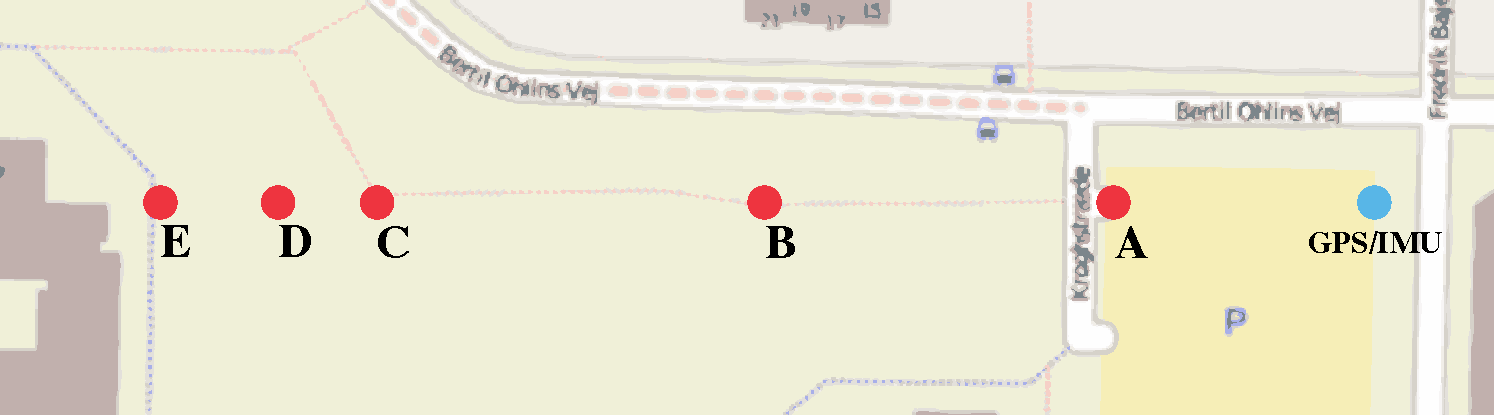
\includegraphics[width=\textwidth]{img/measpoint}
			\caption{Depiction Where the measurements have been taken.}
			\label{fig:mpoint}
		\end{center}
\end{figure}

The probability of receiving a package $p$ is computed as the devision of the number of lost packages and the number of received packages. This gives the following:
\begin{align}
p = 1 - \frac{\text{number of lost packets}}{\text{number of packets}} = \frac{n_\text{l}}{n_\text{r}}
\end{align}

The results are listed in table \vref{tab:res_pack}, which respresents the number of packets received, the number lost and the probability of succes with receiving GPS packages.\\

\begin{tabular}{l*{6}{c}r}
Distance [$m$]             & packets [$n_\text{r}$] & lost packets [$n_\text{l}$] & Probability [$p_\text{gps}$]\\
\hline
2 metres & 244 & 1 & 0.9959\\
47 metres & 217 & 16 & 0.9263\\
95 metres & 227 & 34 & 0.8502\\
156 metres & 218 & 16 & 0.9266\\
169 metres & 225 & 3 & 0.9867\\
189 metres & 221 & 30 & 0.8643\\
\label{tab:res_pack}
\end{tabular}

For the IMU the numbers look like in table \vref{tab:res_pack2}, which also shows that alot more IMU samples have been received due to the higher sampling frequency.\\
\begin{tabular}{l*{6}{c}r}
Distance [$m$] &  packets [$n_\text{r}$] & lost packets [$n_\text{l}$] & Probability [$p_\text{imu}$]\\
\hline
2 metres & 5264 & 1 & 0.9998\\
47 metres & 4813 & 272 & 0.9435\\
95 metres & 4692 & 415 & 0.9116\\
156 metres & 4795 & 382 & 0.9203\\
169 metres & 4838 & 27 & 0.9944\\
189 metres & 4835 & 634 & 0.8689\\
\label{tab:res_pack2}
\end{tabular}

This gives the following distributions for the two packets which can be given as the worst case scenario (to ensure that the actual performance will only be better) - which gives the following distributions:
\begin{align}
\gamma_\text{gps}[n] = 
\left\{ 
  \begin{array}{l l}
    0.8502 & \quad \text{for}\,\, \gamma[n] = 1\\
    0.1498 & \quad \text{for}\,\, \gamma[n] = 0
  \end{array} \right.\\
  \gamma_\text{imu}[n] = 
\left\{ 
  \begin{array}{l l}
    0.8689 & \quad \text{for}\,\, \gamma[n] = 1\\
    0.1311 & \quad \text{for}\,\, \gamma[n] = 0
  \end{array} \right.
\end{align}
As seen on the example, the two distributions sets some requirements to the ship, as a 1 second kill-switch would cut the system out constantly as $n \to \infty$. 

\section{Packet clustering}
To determine if the packets loss are clustered (eg. due to the bigger GPS packets) the below figure determines where the biggest amount of packets are lost. 

\begin{figure}[htbp]
		\begin{center}
			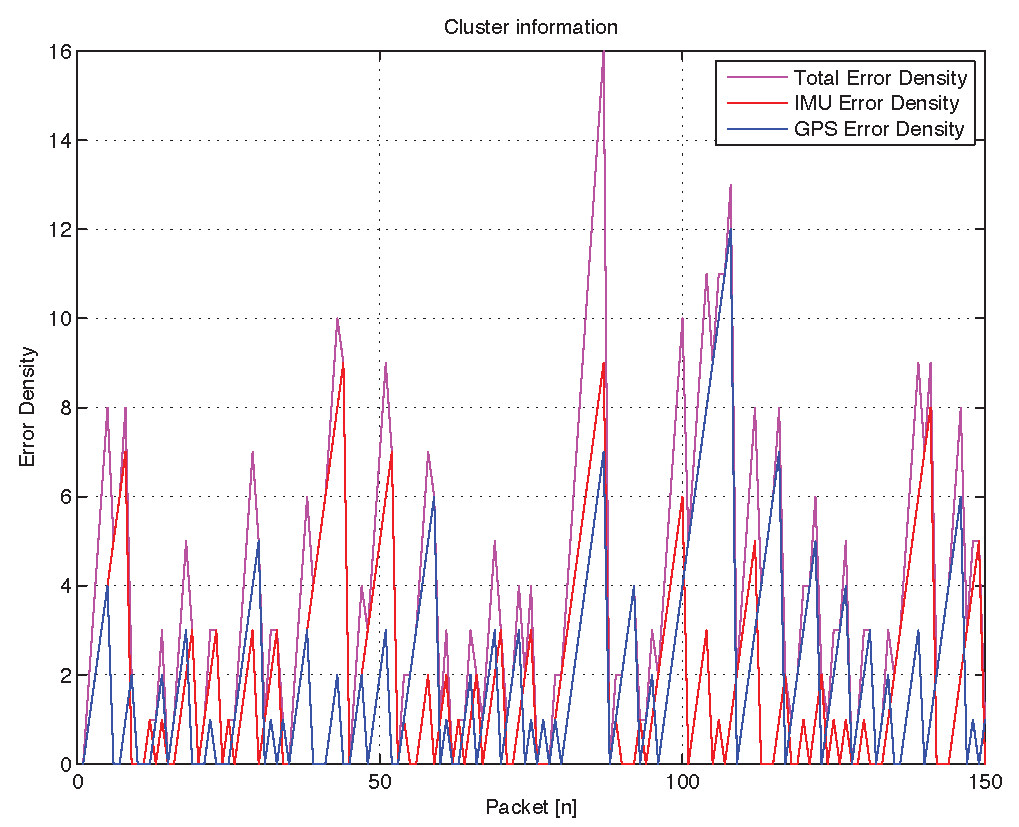
\includegraphics[width=\textwidth]{img/cluster}
			\caption{The red represents the error density of the IMU packets, the blue represents the density of the GPS packets and the magenta is the sum of these. When this grows large it is either due to one of the packets being large or them both. }
			\label{fig:cluster}
		\end{center}
\end{figure}

Figure \vref{fig:cluster} illustrates the density of lost packages. 

The mean packet loss is derived to be: whilst the variance is given as: 

Test results show that the communication link at a distance of X metres begin to have quite a high loss ratio with the current equipment mounted on the ship - and so the ship should never be further away, as communication begins to become faulty. To verify if the ship can still navigate without sending packets back and forth. As to verify if the ship can sail without a decent communications link a test have been carried out where the GPS packets were turned off for 

To make a worst case test, a test is carried out where the GPS is turned off for 60 seconds, so only the IMU goes through. 

To get a precise measurement of the probability, a test in a more controlled environment could be carried out. This could improve on the errors that occur in the signal. 